% !TeX root = ../main.tex

\section{Introduction}
The earliest algorithms developed in recommender systems were
neighborhood-based collaborative filtering algorithms. These algorithms
utilize the similarities between either of users or items, based on the ratings.
The data in a recommender system can be presented as a matrix called the ratings
matrix($\mathcal{R}$).
\begin{table}[H]
\centering
\begin{tabular}{ |c|c|c|c|c| }
\hline
\diagbox{$User$}{$Item$} & \textbf{$Item_1$} & \textbf{$Item_2$} & \textbf{$Item_3$} & \textbf{$Item_4$} \\
\hline
\textbf{$User_1$} & 5 & 2 & \textbf{?} & 3 \\
\hline
\textbf{$User_2$} & 1 & \textbf{?} & 4 & 2 \\
\hline
\textbf{$User_3$} & \textbf{?}  & 3 & 5 & 4 \\
\hline
\textbf{$User_4$} & 5 & 2 & 3 &  \textbf{?} \\
\hline
\textbf{$User_5$} & 1 & \textbf{?}  & 2 & 4 \\
\hline
\textbf{$User_6$} & 3 & 5 & \textbf{?}  & 3 \\
\hline
\textbf{$User_7$} & 3 & 1 & \textbf{?}  & 5 \\
\hline
\end{tabular}
\caption{Ratings Matrix}
\label{table:Ratings Matrix}
\end{table}

\justify
The rows of the matrix represent users($\mathcal{U}$) and the
columns represent items($\mathcal{I}$). A rating($r$) is a number in this case an integer in
the range [1 - 5] that a user has given to an item, where 1 means that
the users totally disliked the item and 5 that the user totally liked the item. The missing ratings are those
that the users haven't reviewed yet and also where the rating predictions apply.
The known ratings are used for the similarity computations and therefore for
the rating predictions. There are two types of neighborhood-based algorithms:
\begin{itemize}
	\item \textbf{User-based CF:}  This type utilizes the ratings matrix
	row-wise meaning the recommender system is trying to find similar patterns
	between users. Given the ratings matrix, to predict the rating that
	$User_4$ would give to $Item_4$ first it would try to find users
	that have rated $Item_4$ and out of these users to select those
	(also called nearest neighbors) who have liked similar items with $User_4$
	in the past. Then based on the most similar nearest neighbors to $User_4$
	a prediction would be computed as an aggregation of the target user's nearest neighbors
	ratings. This method assumes two things. The first one is that if users
	had similar interests in the past they will have similar interests in the future.
	The second assumption is that user preferences remain stable and
	consistent over time. \citep{Jannach}

	\item \textbf{Item-based CF:} This type utilizes the ratings matrix
	column-wise and it is trying to find patterns between the items. Again
	from the ratings matrix, to predict the rating that $User_4$ would give to
	$Item_4$ it would try to find other items, that this user has rated. The
	rating prediction would  be an aggregation of the ratings of the most similar
	items between those and $Item_4$. Item-based CF is considered a more viable approach in
	real cases for two reasons. The first reason is that the items are usually far
	less than the users	in the system. This reduces both the computation
	time and storage needed for the similarities. The second reason is that
	users tend to rate a small proportion of items, which distorts the
	user similarities because of the sparseness. Instead, each item accumulates more
	ratings, as items are less than users, which makes item-based
	similarities more reliable.\citep{sarwar2001item}
\end{itemize}
The main advantages of the neighborhood-based algorithms\citep{Ricci} are:
\begin{itemize}
	\item \textbf{Simplicity:} To implement a neighborhood-based algorithm
	the only factor that is considered is the ratings in the matrix in order
	to find similarities.
	\item \textbf{Justifiability:} It is very clear how the rating
	predictions were computed and why it makes sense from the data as the
	similarities that gave these predictions can be provided to the users, so
	as to justify their relevance.
	\item \textbf{Efficiency:} The training cost in neighbor-based methods
	consists only of the similarity pre-computations between users or items
	which can be computed offline in the ratings matrix which is much cheaper than
	most model-based training. Offline learning means that the system
	will not adapt immediately to any change. Instead it must recompute
	the similarities from scratch. Moreover, storing only the nearest neighbors
	in memory requires only a little use of RAM, instead of storing every user
	which could form a similarity with the active user.
	\item \textbf{Stability:} In large scale recommenders systems, typically in
	item-based approach, it is observed that the addition of users, items and ratings slightly
	affect the decisions of the system after item similarities have been computed.
	That means that the RS would not need further re-training to make better recommendations.
	Also when new items enter the system, they can be trained solely without affecting other items'
	existing similarities.
\end{itemize}

As discussed in the previous chapter, neighborhood-based algorithms suffer from the sparsity of
the ratings matrix. When the similarities are calculated from
only a few common ratings between, e.g. two items, this often leads to
an ambiguous similarity score that can produce spurious predictions.
Another symptom of sparseness is that sometimes no similarities between
items or users can be found and this inability leaves those items or users
without neighbors. Thus, without neighbors they won't participate in
the rating prediction process which means that the RS won't be able to provide
recommendations for those entities.

In \autoref{sec:2.2} different similarity metrics will be discussed.
In \autoref{sec:2.3} The KNN algorithm will be explained and a full example will be
demonstrated for further clarification.

\section{Similarity Metrics}\label{sec:2.2}
The most important part in a neighborhood-based CF approach is the computation of
the similarities which, as we discussed above, can be user-based or item-based.
Below, different similarity metrics will be mentioned. Some of them are widely known metrics
in the literature. These are Cosine Similarity, Pearson Correlation Coefficient,
Adjusted Cosine Similarity, Mean Absolute Difference, Mean Squared Difference and
Jaccard Coefficient. The rest of them are modifications
of the original metrics that we introduce and do not exist in the literature.
These are the Modified Cosine Similarity, Modified Adjusted Cosine Similarity,
Modified Pearson Correlation Coefficient 1 and Modified Pearson Correlation Coefficient 2.
Some of the widely known similarity metrics have been introduced as a user-based approach
and others as item-based. In this thesis we will define each similarity metric both for
user-based and item-based. Also we will assume that the values of the ratings matrix
consist of integers in the interval [1, 5] in order to define the interval for
each similarity metric.
\subsection{Mathematical Notation}
For consistency over the similarity metrics formulas that will be defined next,
a global mathematical notation is used for the rest of this section.
Uppercase $\mathcal{I}$ is used to denote the set of items in the system.
The notation $\mathcal{I}_u$ is the set of items that have been rated by
user $u$, $\mathcal{I}_v$ is the set of items that have been rated by
user $v$ and $\mathcal{I}_{uv}$ is $\mathcal{I}_u \cap \mathcal{I}_v$ that is the set of items that users $u$ and $v$ have
rated in common.
Similarly, uppercase $\mathcal{U}$ is used to denote the set of users in the system.
$\mathcal{U}_i$ is the set of users that have rated
item $i$, $\mathcal{U}_j$ is the set of users that have rated
item $j$ and $\mathcal{U}_{ij}$ is $\mathcal{U}_i \cap \mathcal{U}_j$ that is the set of users that have rated both
items $i$ and $j$. The notation $\mathopen|\mathcal{I}_{u}\mathclose|$ denotes
the number of items user $u$ has rated, $\mathopen|\mathcal{I}_{v}\mathclose|$
denotes the number of items user $v$ has rated, and $\mathopen|\mathcal{I}_{uv}\mathclose|$
is the number of items that users $u$ and $v$ have rated in common. Likewise,
$\mathopen|\mathcal{U}_{i}\mathclose|$ denotes the number of users that have
rated item $i$, $\mathopen|\mathcal{U}_{j}\mathclose|$ denotes the number of users that have rated
item $j$, and $\mathopen|\mathcal{U}_{ij}\mathclose|$ is the number of users that
have both rated items $i$ annd $j$.
$r_{ui}$ is the rating that user $u$ gave to item $i$ and
$r_{vi}$ the rating that user $v$ gave to item $i$.
$r_{iu}$ is the rating item $i$ received from user $u$ and
$r_{ju}$ the rating item $j$ received from user $u$.

\subsection{Cosine similarity}
Cosine similarity is a metric that measures the cosine of the angle that two vectors form.
This metric can take any value in the interval [-1, 1], but specifically for our
own case where the ratings matrix is defined in the interval [1, 5], this
metric is defined in the interval [0, 1].\\\\
User-based cosine similarity between users $u$ and $v$ is defined as:
\begin{equation}\label{eq:cosine}
    cos(u,v) = \frac{\sum_{i \in \mathcal{I}_{uv}}r_{ui}r_{vi}}
		    {\sqrt{\sum_{i \in \mathcal{I}_{u}}r_{ui}^2}
		     \sqrt{\sum_{i \in \mathcal{I}_{v}}r_{vi}^2}}
\end{equation}
The largest the similarity value the higher is chance that these users rate by the same way.
A zero similarity score indicates that $u$ and $v$ have no items in common and therefore
they have no similarity.\\\\
From \autoref{table:Ratings Matrix}, the cosine similarity
between $User_1$ and $User_3$ would thus be computed as follows:
\begin{align*}
cos(User_1,User_3) = \frac{2*3 + 3*4}
						{\sqrt{5^2 + 2^2 + 3^2} * \sqrt{3^2 + 5^2 + 4^2}} = 0.4129
\end{align*}
Similarly, instead of using the row vectors to calculate the similarity between users,
column vectors can be used to calculate the similarity between item pairs.\\\\
Item-based cosine similarity between items $i$ and $j$ is defined as:
\begin{equation}
    cos(i,j) = \frac{\sum_{u \in \mathcal{U}_{ij}}r_{iu}r_{ju}}
		    {\sqrt{\sum_{u \in \mathcal{U}_{i}}r_{iu}^2}
		     \sqrt{\sum_{u \in \mathcal{U}_{j}}r_{ju}^2}}
\end{equation}
Again from \autoref{table:Ratings Matrix}, the cosine similarity
between $Item_2$ and $Item_3$ would thus be computed as follows:
\begin{align*}
cos(Item_2,Item_3) = \frac{3*5 + 2*3}
						{\sqrt{2^2 + 3^2 + 2^2 + 5^2 + 1^2} * \sqrt{4^2 + 5^2 + 3^2 + 2^2}} = 0.4358
\end{align*}
\subsection{Modified Cosine Similarity}
Modified cosine similarity differs from the standard cosine similarity in the
sense that the computations in the denominator apply only to the common items
between $u$ and $v$.
Its values are defined in the interval [0, 1].\\\\
User-based modified cosine similarity between users $u$ and $v$ is defined as:
\begin{equation}\label{eq:modified_cosine}
    MC(u,v) = \frac{\sum_{i \in \mathcal{I}_{uv}}r_{ui}r_{vi}}
		   {\sqrt{\sum_{i \in \mathcal{I}_{uv}}r_{ui}^2}
                    \sqrt{\sum_{i \in \mathcal{I}_{uv}}r_{vi}^2}}
\end{equation}
From \autoref{table:Ratings Matrix}, MC
between $User_1$ and $User_3$ would thus be computed as follows:
\begin{align*}
MC(User_1,User_3) = \frac{2*3 + 3*4}
					   {\sqrt{2^2 + 3^2} * \sqrt{3^2 + 4^2}} = 0.9984
\end{align*}
We can reverse the above formula in order to calculate the similarities
in terms of items.\\
Item-based modified cosine similarity between items $i$ and $j$ is defined as:
\begin{equation}
    MC(i,j) = \frac{\sum_{u \in \mathcal{U}_{ij}}r_{iu}r_{ju}}
   {\sqrt{\sum_{u \in \mathcal{U}_{ij}}r_{iu}^2}
            \sqrt{\sum_{u \in \mathcal{U}_{ij}}r_{ju}^2}}
\end{equation}
From \autoref{table:Ratings Matrix}, MC
between $Item_2$ and $Item_3$ would thus be computed as follows:
\begin{align*}
MC(Item_2,Item_3) = \frac{3*5 + 2*3}
						{\sqrt{3^2 + 2^2} * \sqrt{5^2 + 3^2}} = 0.9988
\end{align*}
\subsection{Adjusted Cosine Similarity}
Adjusted cosine similarity was originally created as an
item-based approach. The reason for that was because each item vector consists of
users who have different rating behaviors and cosine similarity did not
take into account these disparities. That means that a user could use the
rating 3 for items that really liked and 1 for items that really disliked while
another user could give a 5 rating to items that really liked and 1 to them that really
disliked. Adjusted cosine similarity is computed by looking into the co-rated items
($\mathcal{U}_{ij}$) only. It normalizes each user's rating behavior by
subtracting the corresponding user's mean value \citep{sarwar2001item}.
Adjusted cosine similarity values are defined in the interval [-1, 1].
The value -1 means perfect dissimilarity between two items while the value 1 means
perfect similarity. The zero value means there is no similarity between these items.\\\\
Item-based adjusted cosine similarity between items $i$ and $j$ is defined as:
\begin{equation}\label{eq:adjusted_cosine}
    \begin{split}
    &AC(i,j) = \frac{\sum_{u \in \mathcal{U}_{ij}}(r_{iu}-\bar{r_{u}})(r_{ju}-\bar{r_{u}})}
		    {\sqrt{\sum_{u \in \mathcal{U}_{ij}}(r_{iu}-\bar{r_{u}})^2}
                     \sqrt{\sum_{u \in \mathcal{U}_{ij}}(r_{ju}-\bar{r_{u}})^2}} \\\\
    &\bar{r_{u}} = \frac{\sum_{i \in \mathcal{I}_u}r_{ui}}
 		        {\mathopen|\mathcal{I}_u\mathclose|}
    \end{split}
\end{equation}
where,
\begin{itemize}
	\item[] $\bar{r_u}$ is the mean value of user $u$ for each $u \in \mathcal{U}_{ij}$
\end{itemize}
From \autoref{table:Ratings Matrix}, AC
between $Item_2$ and $Item_3$ would thus be computed as follows:
\begin{align*}
	\begin{split}
		&\bar{r}_{User_3} = \frac{3 + 5 + 4}{3} = 4\\
		&\bar{r}_{User_4} = \frac{5 + 2 + 3}{3} = 3.33
	\end{split}
\end{align*}
$$AC(Item_2,Item_3) = \frac{(3 - 4)*(5 - 4) + (2 - 3.33)*(3 - 3.33)}
						 {\sqrt{(3 - 4)^2 + (2 - 3.33)^2}*
						  \sqrt{(5 - 4)^2 + (3 - 3.33)^2}} = −0.3202$$
The result $-0.3202$ means that $Item_2$ and $Item_3$ are somewhat dissimilar.\\\\
We could use the same reasoning adjusted cosine was build on,
to look at this formula from a user-based perspective. That is, if an item's
lowest rating is 3 and its highest rating is 5, that means that it is treated
differently than an item that its lowest rating is 1 and the highest 4.
Therefore, we could have each co-rated item, by two users, mean centered by the corresponding item
and calculate a user-based adjusted cosine similarity.\\\\
User-based adjusted cosine similarity between users $u$ and $v$ is defined as:
\begin{equation}
\begin{split}
    &AC(u,v) = \frac{\sum_{i \in \mathcal{I}_{uv}}(r_{ui}-\bar{r_{i}})(r_{vi}-\bar{r_{i}})}
		    {\sqrt{\sum_{i \in \mathcal{I}_{uv}}(r_{ui}-\bar{r_{i}})^2}
                     \sqrt{\sum_{i \in \mathcal{I}_{uv}}(r_{vi}-\bar{r_{i}})^2}} \\\\
    &\bar{r_{i}} = \frac{\sum_{u \in \mathcal{U}_i}r_{iu}}
 		        {\mathopen|\mathcal{U}_i\mathclose|}
\end{split}
\end{equation}
where,
\begin{itemize}
	\item[] $\bar{r_i}$ is the mean value of item $i$ for each $i \in \mathcal{I}_{uv}$
\end{itemize}
From \autoref{table:Ratings Matrix}, AC
between $User_1$ and $User_3$ would thus be computed as follows:
\begin{align*}
	\begin{split}
		&\bar{r}_{Item_2} = \frac{2 + 3 + 2 + 5 + 1}{5} = 2.6\\
		&\bar{r}_{Item_4} = \frac{3 + 2 + 4 + 4 + 3 + 5}{6} = 3.5
	\end{split}
\end{align*}
$$AC(User_1,User_3) = \frac{(2 - 2.6)*(3 - 2.6) + (3 - 3.5)*(4 - 3.5)}
						 {\sqrt{(2 - 2.6)^2 + (3 - 3.5)^2}*
						  \sqrt{(3 - 2.6)^2 + (4 - 3.5)^2}} = −0.9798$$
$User_1$ and $User_3$ are almost perfectly dissimilar.
\subsection{Modified Adjusted Cosine Similarity}
A modification to adjusted cosine similarity that we implemented was to
use every user corresponding to $i$ and $j$ instead of using
only the users that have rated both items in the denominator. Its values are also in the interval [-1, 1].\\\\
Item-based modified adjusted cosine similarity between items $i$ and $j$ is defined as:
\begin{equation}
\begin{split}
&MAC(i,j) = \frac{\sum_{u \in \mathcal{U}_{ij}}(r_{iu}-\bar{r_{u}})(r_{ju}-\bar{r_{u}})}
				 {\sqrt{\sum_{u \in \mathcal{U}_{i}}(r_{iu}-\bar{r_{u}})^2}
				  \sqrt{\sum_{u \in \mathcal{U}_{j}}(r_{ju}-\bar{r_{u}})^2}} \\\\
&\bar{r_{u}} = \frac{\sum_{i \in \mathcal{I}_u}r_{ui}}
					{\mathopen|\mathcal{I}_u\mathclose|}
\end{split}
\end{equation}
where,
\begin{itemize}
	\item[] $\bar{r_u}$ is the mean value of user $u$ for each $u \in \mathcal{U}_{ij}$ in the numerator
	\item[] $\bar{r_u}$ is the mean value of user $u$ for each $u \in \mathcal{U}_{i}$ and $u \in \mathcal{U}_{j}$ respectively in the denominator
\end{itemize}
From \autoref{table:Ratings Matrix}, MAC
between $Item_2$ and $Item_3$ would thus be computed as follows:
\footnotesize
\begin{align*}
	\begin{split}
		&\bar{r}_{User_1} = \frac{5 + 2 + 3}{3} = 3.33\\
		&\bar{r}_{User_2} = \frac{1 + 4 + 2}{3} = 2.33\\
		&\bar{r}_{User_3} = \frac{3 + 5 + 4}{3} = 4\\
		&\bar{r}_{User_4} = \frac{5 + 2 + 3}{3} = 3.33\\
		&\bar{r}_{User_5} = \frac{1 + 2 + 4}{3} = 2.33\\
		&\bar{r}_{User_6} = \frac{3 + 5 + 3}{3} = 3.66\\
		&\bar{r}_{User_7} = \frac{3 + 1 + 5}{3} = 3\\\\
&MAC(Item_2,Item_3) = \\&\frac{(3 - 4)*(5 - 4) + (2 - 3.33)*(3 - 3.33)}
						 {\sqrt{(2 - 3.33)^2 + (3 - 4)^2 + (2 - 3.33)^2 + (5 - 3.66)^2 + (1 - 3)^2}*
						  \sqrt{(4 - 2.33)^2 + (5 - 4)^2 + (3 - 3.33)^2 + (2 - 2.33)^2}} \\&= −0,0872
  \end{split}
\end{align*}
\normalsize
Compared to item-based AC the item-based MAC between $Item_2$ and $Item_3$ still generates
a negative similarity but it is very close to zero this time as it takes into account each
item's vector length.\\\\
As previously mentioned a user-based approach can also be implemented.\\
User-based modified adjusted cosine similarity between users $u$ and $v$ is defined as:
\begin{equation}\label{eq:modified_adjusted_cosine}
\begin{split}
    &MAC(u,v) = \frac{\sum_{i \in \mathcal{I}_{uv}}(r_{ui}-\bar{r_{i}})(r_{vi}-\bar{r_{i}})}
                     {\sqrt{\sum_{i \in \mathcal{I}_{u}}(r_{ui}-\bar{r_{i}})^2}
                      \sqrt{\sum_{i \in \mathcal{I}_{v}}(r_{vi}-\bar{r_{i}})^2}} \\\\
    &\bar{r_{i}} = \frac{\sum_{u \in \mathcal{U}_i}r_{iu}}
                        {\mathopen|\mathcal{U}_i\mathclose|}
\end{split}
\end{equation}
where,
\begin{itemize}
	\item[] $\bar{r_i}$ is the mean value of user $u$ for each $u \in \mathcal{I}_{uv}$ in the numerator
	\item[] $\bar{r_i}$ is the mean value of user $u$ for each $u \in \mathcal{I}_{u}$ and $u \in \mathcal{I}_{v}$ respectively in the denominator
\end{itemize}
From \autoref{table:Ratings Matrix}, MAC
between $User_1$ and $User_3$ would thus be computed as follows:
\begin{align*}
	\begin{split}
		&\bar{r}_{Item_1} = 3\\
		&\bar{r}_{Item_2}  = 2.6\\
		&\bar{r}_{Item_3} = 3.5\\
		&\bar{r}_{Item_4} = 3.5\\\\
MAC(User_1,User_3) &= \frac{(2 - 2.6)*(3 - 2.6) + (3 - 3.5)*(4 - 3.5)}
						 {\sqrt{(5 - 3)^2 + (2 - 2.6)^2 + (3 - 3.5)^2}*
						  \sqrt{(3 - 2.6)^2 + (5 - 3.5)^2 + (4 - 3.5)^2}} \\&= −0.1399
  \end{split}
\end{align*}
Compared to user-based AC, the user-based MAC between $User_1$ and $User_3$ still generates
a negative similarity but it is far weaker than AC's as it takes into account the length of
each user's vector.
\subsection{Pearson Correlation Coefficient}
Users do not always rate in the same way. One user might never use a rating of 5
for items that really likes.
Another user might never rate an item below 3 for items that really dislikes.
A third user might only use a rating of 4 despite of how much he liked an item.
This means is that most of the users have a particularity in their
ratings. Due to this user behavior, it is difficult to understand the similarity
based on the actual rating. The Pearson correlation coefficient
computes the linear correlation between two users, to alleviate this problem. Linear correlation is
defined as the proportion of dependence between two variables X and Y.
Regarding the similarity between two users, the Pearson correlation coefficient can also be
thought of as the covariance between two users A and B divided by the standard deviation of
$User_A$ multiplied by the standard deviation of $User_B$.\\\\
User-based Pearson correlation coefficient between users $u$ and $v$ is defined as:
\begin{equation}\label{eq:pearson}
\begin{split}
    &PCC(u,v) = \frac{\sum_{i \in \mathcal{I}_{uv}}(r_{ui}-\bar{r_{u}})(r_{vi}-\bar{r_{v}})}
                     {\sqrt{\sum_{i \in \mathcal{I}_{uv}}(r_{ui}-\bar{r_{u}})^2}
                      \sqrt{\sum_{i \in \mathcal{I}_{uv}}(r_{vi}-\bar{r_{v}})^2}} \\\\
    &\bar{r_{u}} = \frac{\sum_{i \in \mathcal{I}_u}r_{ui}}
                        {\mathopen|\mathcal{I}_u\mathclose|}\\
    &\bar{r_{v}} = \frac{\sum_{i \in \mathcal{I}_v}r_{vi}}
                        {\mathopen|\mathcal{I}_v\mathclose|}
\end{split}
\end{equation}
where,
\begin{itemize}
	\item[] $\bar{r_u}$ is the mean value of user $u$
	\item[] $\bar{r_v}$ is the mean value of user $v$
\end{itemize}
The PCC varies between -1 and 1 and based on its value two objects inspected for correlation can
be classified as:
\begin{itemize}
	\item Positively correlated, when $PCC > 0$
	\item Negatively correlated, when $PCC < 0$
	\item Uncorrelated,  when $PCC = 0$
\end{itemize}
From \autoref{table:Ratings Matrix}, PCC
between $User_1$ and $User_3$ would thus be computed as follows:
\begin{align*}
	\begin{split}
		&\bar{r}_{User_1} = 3.33\\
		&\bar{r}_{User_3} = 4\\\\
		PCC(User_1,User_3) &= \frac{(2 - 3.33) * (3 - 4) + (3 - 3.33) * (4 - 4)}
								  {\sqrt{(2 - 3.33)^2 + (3 - 3.33)^2} *
								   \sqrt{(3 - 4)^2 + (4 - 4)^2}} = 0.9705
	\end{split}
\end{align*}
Thus $User_1$ and $User_3$ have a strong positive correlation.\\\\
PCC was initially used as a user-based approach\citep{shardanand1995social} but we will
reverse it for item-based computations in order to measure the correlation between the items.\\\\
Item-based Pearson correlation coefficient between items $i$ and $j$ is defined as:
\begin{equation}
	\begin{split}
	&PCC(i,j) = \frac{\sum_{u \in \mathcal{U}_{ij}}(r_{iu}-\bar{r_{i}})(r_{ju}-\bar{r_{j}})}
					 {\sqrt{\sum_{u \in \mathcal{U}_{ij}}(r_{iu}-\bar{r_{i}})^2}
					  \sqrt{\sum_{u \in \mathcal{U}_{ij}}(r_{ju}-\bar{r_{j}})^2}} \\\\
	&\bar{r_{i}} = \frac{\sum_{u \in \mathcal{U}_i}r_{iu}}
						{\mathopen|\mathcal{U}_i\mathclose|}\\
	&\bar{r_{j}} = \frac{\sum_{u \in \mathcal{U}_j}r_{ju}}
						{\mathopen|\mathcal{U}_j\mathclose|}
\end{split}
\end{equation}
where,
\begin{itemize}
	\item[] $\bar{r_i}$ is the mean value of item $i$
	\item[] $\bar{r_j}$ is the mean value of item $j$
\end{itemize}
From \autoref{table:Ratings Matrix}, PCC
between $Item_2$ and $Item_3$ would thus be computed as follows:
\begin{align*}
	\begin{split}
		&\bar{r}_{Item_2} = 2.6\\
		&\bar{r}_{Item_3} = 3.5\\\\
		PCC(Item_2,Item_3) &= \frac{(3 - 2.6) * (5 - 3.5) + (2 - 2.6) * (3 - 3.5)}
								  {\sqrt{(3 - 2.6)^2 + (2 - 2.6)^2} *
								   \sqrt{(5 - 3.5)^2 + (3 - 3.5)^2}} = 0.7893
	\end{split}
\end{align*}
Thus $Item_2$ and $Item_3$ have a strong positive correlation.
\subsection{Modified Pearson Correlation Coefficient 1}
The first modification to PCC that we implemented was to average only the ratings that
two users have in common. Its values are in the interval [-1, 1].\\\\
User-based modified Pearson correlation coefficient 1 between users $u$ and $v$ is defined as:
\begin{equation}\label{eq:pearson_1}
\begin{split}
    &MPCC1(u,v) = \frac{\sum_{i \in \mathcal{I}_{uv}}(r_{ui}-\tilde{r_{u}})(r_{vi}-\tilde{r_{v}})}
                       {\sqrt{\sum_{i \in \mathcal{I}_{uv}}(r_{ui}-\tilde{r_{u}})^2}
                        \sqrt{\sum_{i \in \mathcal{I}_{uv}}(r_{vi}-\tilde{r_{v}})^2}} \\\\
    &\tilde{r_{u}} = \frac{\sum_{i \in \mathcal{I}_{uv}}r_{ui}}
                          {\mathopen|\mathcal{I}_{uv}\mathclose|}\\
    &\tilde{r_{v}} = \frac{\sum_{i \in \mathcal{I}_{uv}}r_{vi}}
                          {\mathopen|\mathcal{I}_{uv}\mathclose|}
\end{split}
\end{equation}
where,
\begin{itemize}
	\item[] $\tilde{r_u}$ is the mean value of user $u$ using only the co-rated items with user $v$
	\item[] $\tilde{r_v}$ is the mean value of user $v$ using only the co-rated items with user $u$
\end{itemize}
From \autoref{table:Ratings Matrix}, MPCC1
between $User_1$ and $User_3$ would thus be computed as follows:
\begin{align*}
	\begin{split}
		&\tilde{r}_{User_1} = \frac{2 + 3}{2} = 2.5\\
		&\tilde{r}_{User_3} = \frac{3 + 4}{2} = 3.5\\\\
		MPCC1(User_1,User_3) &= \frac{(2 - 2.5) * (3 - 3.5) + (3 - 2.5) * (4 - 3.5)}
								  {\sqrt{(2 - 2.5)^2 + (3 - 2.5)^2} *
								   \sqrt{(3 - 3.5)^2 + (4 - 3.5)^2}} = 1
	\end{split}
\end{align*}
Compared to user-based PCC, the user-based MPCC1 between $User_1$ and $User_3$
using the modified mean values yields a perfect correlation.\\\\
Item-based modified Pearson correlation coefficient 1 between items $i$ and $j$ is defined as:
\begin{equation}
	\begin{split}
	&MPCC1(i,j) = \frac{\sum_{u \in \mathcal{U}_{ij}}(r_{iu}-\tilde{r_{i}})(r_{ju}-\tilde{r_{j}})}
					 {\sqrt{\sum_{u \in \mathcal{U}_{ij}}(r_{iu}-\tilde{r_{i}})^2}
					  \sqrt{\sum_{u \in \mathcal{U}_{ij}}(r_{ju}-\tilde{r_{j}})^2}} \\\\
	&\tilde{r_{i}} = \frac{\sum_{u \in \mathcal{U}_{ij}}r_{iu}}
						{\mathopen|\mathcal{U}_{ij}\mathclose|}\\
	&\tilde{r_{j}} = \frac{\sum_{u \in \mathcal{U}_{ij}}r_{ju}}
						{\mathopen|\mathcal{U}_{ij}\mathclose|}
\end{split}
\end{equation}
where,
\begin{itemize}
	\item[] $\tilde{r_i}$ is the mean value of item $i$ using only the common user ratings with item $j$
	\item[] $\tilde{r_j}$ is the mean value of item $j$ using only the common user ratings with item $i$
\end{itemize}
From \autoref{table:Ratings Matrix}, MPCC1
between $Item_2$ and $Item_3$ would thus be computed as follows:
\begin{align*}
	\begin{split}
		&\tilde{r}_{Item_2} = \frac{3 + 2}{2} = 2.5\\
		&\tilde{r}_{Item_3} = \frac{5 + 3}{2} = 4\\\\
		MPCC1(Item_2,Item_3) &= \frac{(3 - 2,5) * (5 - 4) + (2 - 2,5) * (3 - 4)}
								  {\sqrt{(3 - 2,5)^2 + (2 - 2,5)^2} *
								   \sqrt{(5 - 4)^2 + (3 - 4)^2}} = 1
	\end{split}
\end{align*}
Compared to item-based PCC, item-based MPCC1 between $Item_2$ and $Item_3$
using the modified mean values yields a perfect correlation.
\subsection{Modified Pearson Correlation Coefficient 2}
The second modification to PCC is to change the denominator
in a sense that it includes all the items corresponding to $u$ and $v$ respectively.
Its values are also in the interval [-1, 1].\\\\
User-based modified Pearson correlation coefficient 2 between users $u$ and $v$ is defined as:
\begin{equation}\label{eq:pearson_2}
\begin{split}
    &MPCC2(u,v) = \frac{\sum_{i \in \mathcal{I}_{uv}}(r_{ui}-\bar{r_{u}})(r_{vi}-\bar{r_{v}})}
                       {\sqrt{\sum_{i \in \mathcal{I}_{u}}(r_{ui}-\bar{r_{u}})^2}
                        \sqrt{\sum_{i \in \mathcal{I}_{v}}(r_{vi}-\bar{r_{v}})^2}} \\\\
    &\bar{r_{u}} = \frac{\sum_{i \in \mathcal{I}_u}r_{ui}}
                        {\mathopen|\mathcal{I}_u\mathclose|}\\
    &\bar{r_{v}} = \frac{\sum_{i \in \mathcal{I}_v}r_{vi}}
                        {\mathopen|\mathcal{I}_v\mathclose|}
\end{split}
\end{equation}
where,
\begin{itemize}
	\item[] $\bar{r_u}$ is the mean value of user $u$
	\item[] $\bar{r_v}$ is the mean value of user $v$
\end{itemize}
From \autoref{table:Ratings Matrix}, MPCC2
between $User_1$ and $User_3$ would thus be computed as follows:
\begin{align*}
	\begin{split}
		&\bar{r}_{User_1} = 3.33\\
		&\bar{r}_{User_3} = 4\\\\
		MPCC2(User_1,User_3) &= \frac{(2 - 3.33) * (3 - 4) + (3 - 3.33) * (4 - 4)}
								  {\sqrt{(5 - 3.33)^2 + (2 - 3.33)^2 + (3 - 3.33)^2} *
								   \sqrt{(3 - 4)^2 + (5 - 4)^2 + (4 - 4)^2}} = 0.4353
	\end{split}
\end{align*}
Compared to user-based PCC, the user-based MPCC2 between $User_1$ and $User_3$
retained a positive correlation but it has significantly decreased as it now
takes into account the mean centered length of each user's vector.\\\\
Item-based modified Pearson correlation coefficient 2 between items $i$ and $j$ is defined as:
\begin{equation}
	\begin{split}
	&MPCC2(i,j) = \frac{\sum_{u \in \mathcal{U}_{ij}}(r_{iu}-\bar{r_{i}})(r_{ju}-\bar{r_{j}})}
					 {\sqrt{\sum_{u \in \mathcal{U}_{i}}(r_{iu}-\bar{r_{i}})^2}
					  \sqrt{\sum_{u \in \mathcal{U}_{j}}(r_{ju}-\bar{r_{j}})^2}} \\\\
	&\bar{r_{i}} = \frac{\sum_{u \in \mathcal{U}_i}r_{iu}}
						{\mathopen|\mathcal{U}_i\mathclose|}\\
	&\bar{r_{j}} = \frac{\sum_{u \in \mathcal{U}_j}r_{ju}}
						{\mathopen|\mathcal{U}_j\mathclose|}
\end{split}
\end{equation}
From \autoref{table:Ratings Matrix}, MPCC2
between $Item_2$ and $Item_3$ would thus be computed as follows:
\footnotesize
\begin{align*}
	\begin{split}
		&\bar{r}_{Item_2} = 2.6\\
		&\bar{r}_{Item_3} = 3.5\\\\
		&MPCC2(Item_2,Item_3) = \\&\frac{(3 - 2,6) * (5 - 3,5) + (2 - 2,6) * (3 - 3,5)}
								  {\sqrt{(2 - 2,6)^2 + (3 - 2,6)^2 + (2 - 2,6)^2 + (5 - 2,6)^2 + (1 - 2,6)^2 } *
								   \sqrt{(4 - 3,5)^2 + (5 - 3,5)^2 + (3 - 3,5)^2 + (2 - 3,5)^2 }} = 0,1327
	\end{split}
\end{align*}
\normalsize
Compared to item-based PCC, item-based MPCC2 between $Item_2$ and $Item_3$
retained a positive correlation but it has significantly decreased as it now
takes into account the mean centered length of each item's vector.
\subsection{Mean Squared Difference Similarity}
Mean squared difference\citep{shardanand1995social} is a very simple metric.
\begin{equation}\label{eq:msd}
    MSD(u,v) = \frac{\sum_{i \in \mathcal{I}_{uv}}(r_{ui}-r_{vi})^2}
					{\mathopen|\mathcal{I}_{uv}\mathclose|}
\end{equation}
It designates the degree of dissimilarity between $u$ and $v$ by aggregating the squared differences
between the ratings on the rated items they have in common.
If we reverse the numerator with the denominator it designates the degree
of the similarity between $u$ and $v$ instead.\\\\
User-based mean squared difference similarity between users $u$ and $v$ is defined as:
\begin{equation}
    MSD(u,v) = \frac{\mathopen|\mathcal{I}_{uv}\mathclose|}
                    {\sum_{i \in \mathcal{I}_{uv}}(r_{ui}-r_{vi})^2}
\end{equation}
Its values are in the
interval (0, $\mathopen|\mathcal{I}_{uv}\mathclose|$] in user-based approach. There
is a chance $u$ and $v$ have given exactly the same ratings to each common item between them. In that case MSD similarity
is not defined. That can also be interpreted as $u$ and $v$ have zero dissimilarity.\\\\
From \autoref{table:Ratings Matrix}, MSD
between $User_1$ and $User_3$ would thus be computed as follows:
$$MSD(User_1,User_3) = \frac{2}{(2 - 3)^2 + (3 - 4)^2} = 1$$\\
The maximum similarity between $User_1$ and $User_3$ could be 2. They have
similarity 1 which means that they are rating somewhat by the same way.\\
Item-based mean squared difference similarity between items $i$ and $j$ is defined as:
\begin{equation}
        MSD(i,j) = \frac{\mathopen|\mathcal{U}_{ij}\mathclose|}
                        {\sum_{u \in \mathcal{U}_{ij}}(r_{iu}-r_{ju})^2}
\end{equation}
Its values are in the interval (0, $\mathopen|\mathcal{U}_{ij}\mathclose|$] in item-based approach.\\\\
From \autoref{table:Ratings Matrix}, MSD
between $Item_2$ and $Item_3$ would thus be computed as follows:
$$MSD(Item_2,Item_3) = \frac{2}{(3 - 5)^2 + (2 - 3)^2} = 0.4$$\\
The maximum similarity between $Item_2$ and $Item_3$ could be 2. They have
similarity 0.4 which means that these items are not rated similarly.
\subsection{Mean Absolute Difference Similarity}
Another very similar metric to MSD, is mean absolute difference similarity.
Its difference from the previous method is that it uses the absolute value of
the difference between the ratings of $u$ and $v$ instead of squaring them.
When big differences between the ratings exist, MSD is significantly penalized when squaring the values.
For that reason, using the absolute values helps in moderating the penalty.\\\\
User-based mean absolute difference similarity between users $u$ and $v$ is defined as:
\begin{equation}\label{eq:mad}
    MAD(u,v) = \frac{\mathopen|\mathcal{I}_{uv}\mathclose|}
                    {\sum_{i \in \mathcal{I}_{uv}}\mathopen|r_{ui}-r_{vi}\mathclose|}
\end{equation}
Its values are in the
interval (0, $\mathopen|\mathcal{I}_{uv}\mathclose|$] in user-based approach.\\\\
From \autoref{table:Ratings Matrix}, MAD
between $User_1$ and $User_3$ would thus be computed as follows:
$$MAD(User_1,User_3) = \frac{2}{\mathopen|2 - 3\mathclose| + \mathopen|3 - 4\mathclose|} = 1$$\\\\
Item-based mean absolute difference between items $i$ and $j$ is defined as:
\begin{equation}
MAD(i,j) = \frac{\mathopen|\mathcal{U}_{ij}\mathclose|}
				{\sum_{u \in \mathcal{U}_{ij}}\mathopen|r_{iu}-r_{ju}\mathclose|}
\end{equation}
Its values are in the interval (0, $\mathopen|\mathcal{U}_{ij}\mathclose|$] in item-based approach.\\\\
From \autoref{table:Ratings Matrix}, MAD
between $Item_2$ and $Item_3$ would thus be computed as follows:
$$MAD(Item_2,Item_3) = \frac{2}{\mathopen|3 - 5\mathclose| + \mathopen|2 - 3\mathclose|} = 0.4$$\\
\subsection{Jaccard Coefficient}
Jaccard coefficient measures the overlap of the ratings between two users.
This similarity metric does not use the rating scores that the users have given, but counts
how many common items they have have rated $\mathopen|\mathcal{I}_{uv}\mathclose|$, and how many distinct
items have rated together in total $\mathopen|\mathcal{I}_u\mathclose| \cup \mathopen|\mathcal{I}_v\mathclose| = \mathopen|\mathcal{I}_{u}\mathclose| +
\mathopen|\mathcal{I}_{v}\mathclose| - \mathopen|\mathcal{I}_{uv}\mathclose|$.
Its values are in the interval [0, 1].\\\\
User-based mean absolute difference similarity between users $u$ and $v$ is defined as:
\begin{equation}\label{eq:jaccard}
    J(u,v) = \frac{\mathopen|\mathcal{I}_{uv}\mathclose|}
                  {\mathopen|\mathcal{I}_{u}\mathclose| +
		   \mathopen|\mathcal{I}_{v}\mathclose| -
		   \mathopen|\mathcal{I}_{uv}\mathclose|}
\end{equation}
The table below is an extension of
\autoref{table:Ratings Matrix} for $User_1$ and $User_7$ for demonstration purpose.
\begin{table}[H]
\centering
\begin{tabular}{ |c|c|c|c|c|c|c| }
\hline
\diagbox{User}{Item} & \textbf{$Item_1$} & \textbf{$Item_2$} & \textbf{$Item_3$} & \textbf{$Item_4$} & \textbf{$Item_5$} & \textbf{$Item_6$} \\
\hline
\textbf{$User_1$} & 5 & 2 & \textbf{?}  & 3 & \textbf{?} & \textbf{?}  \\
\hline
\textbf{$User_7$} & 3 & 1 & \textbf{?} & 5 & 2 & 4 \\
\hline
\end{tabular}
\caption{$User_1$ and $User_7$ extended vectors}
\label{table:jaccard_example1}
\end{table}
The first step is to transform the ratings vector between two users to ones and zeros. Ones are the existing ratings and zeros are the ratings that are missing.
\begin{table}[H]
\centering
\begin{tabular}{ |c|c|c|c|c|c|c| }
\hline
\diagbox{User}{Item} & \textbf{$Item_1$} & \textbf{$Item_2$} & \textbf{$Item_3$} & \textbf{$Item_4$} & \textbf{$Item_5$} & \textbf{$Item_6$} \\
\hline
\textbf{$User_1$} & 1 & 1 & 0 & 1 & 0 & 0 \\
\hline
\textbf{$User_7$} & 1 & 1 & 0 & 1 & 1 & 1 \\
\hline
\end{tabular}
\caption{$User_1$ and $User_7$ vectors transformed}
\label{table:jaccard_example2}
\end{table}
Then count the amount of items $u$ and $v$ have rated in common $\mathopen|\mathcal{I}_{uv}\mathclose|$, in this example $User_1$ and $User_7$,
divided by the amount of their items union $\mathopen|\mathcal{I}_u\mathclose| \cup \mathopen|\mathcal{I}_v\mathclose|$.
$$J(User_1,User_7) = \frac{3}{3 + 5 - 3} = 0.6$$\\\\
Similarly, this metric can be used for item-based similarities.\\
Item-based mean absolute difference between items $i$ and $j$ is defined as:
\begin{equation}
J(i,j) = \frac{\mathopen|\mathcal{U}_{ij}\mathclose|}
		  {\mathopen|\mathcal{U}_{i}\mathclose| +
   \mathopen|\mathcal{U}_{j}\mathclose| -
   \mathopen|\mathcal{U}_{ij}\mathclose|}
\end{equation}
From \autoref{table:Ratings Matrix}, Jaccard coefficient
between $Item_2$ and $Item_3$ would thus be computed as follows:
$$J(Item_2,Item_3) = \frac{2}{5 + 4 - 2} = 0.2857$$
\section{K-Nearest Neighbors Algorithm}\label{sec:2.3}
The K-Nearest Neighbors algorithm is a very straightforward technique.
In a user-based KNN setting, in order to predict the rating of $User_A$ for an
$Item_B$ not rated by $User_A$, KNN consists of the following steps:
\begin{itemize}
	\item[] \textbf{Step 1:} Find users that have rated $Item_B$.
	\item[] \textbf{Step 2:} Compute the similarities between $User_A$ and the users that have
	rated $Item_B$.
	\item[] \textbf{Step 3:}  Sort that similarities in descending order.
	\item[] \textbf{Step 4:}  Choose how many neighbors will contribute in the rating
	prediction by selecting the top $\mathcal{K}$ out of all the available
	neighbors($\mathcal{K}$ can be in range [1 - $\mathcal{N}$] where $\mathcal{N}$ is all
	the available neighbors).
	\item[] \textbf{Step 5:} Use an aggregation formula to calculate the rating prediction of
	$User_A$ to $Item_B$. In this case the weighted sum \citep{sarwar2001item} is used.
\begin{equation}\label{nearest_neighbors}
	\hat{r}(User_A,Item_B) = \frac{\sum_{u \in \mathcal{K}}{similarity(User_A,User_u) * r(User_u,Item_B)}}
						    {\sum_{u \in \mathcal{K}}{\mathopen|similarity(User_A,User_u)\mathclose|}}
\end{equation}
\end{itemize}

Thus, the numerator computes the weighted of ratings of the nearest neighbors,
weighted by their similarities with $User_A$.
In a way the similarity can be interpreted as how much users influence
$User_A$. The denominator sums the absolute values of similarities in order to scale the
outcome of the rating prediction in the range [1 - 5]. The absolute value is used because
similarity metrics like Pearson correlation coefficient can take negative values which
will disturb the scaling.\\

In an item-based KNN setting, in order to predict the rating of $User_A$ for an
$Item_B$ not rated by $User_A$, KNN consists of the following steps:
\begin{itemize}
	\item[] \textbf{Step 1:} Find items that have been rated by $User_A$.
	\item[] \textbf{Step 2:} Compute the similarities between $Item_B$ and the items that have
	been rated by $User_A$.
	\item[] \textbf{Step 3:}  Sort that similarities in descending order.
	\item[] \textbf{Step 4:}  Choose how many neighbors will contribute in the rating
	prediction.
	\item[] \textbf{Step 5:} Use an aggregation formula to calculate the rating prediction of
	$User_A$ to $Item_B$.
\begin{equation}\label{nearest_neighbors}
	\hat{r}(User_A,Item_B) = \frac{\sum_{i \in \mathcal{K}}{similarity(Item_B,Item_i) * r(User_A,Item_i)}}
						    {\sum_{i \in \mathcal{K}}{\mathopen|similarity(Item_B,Item_i)\mathclose|}}
\end{equation}
\end{itemize}

There are 4 important things to take into consideration in order to obtain the most accurate
outcome out with the KNN algorithm:
\begin{enumerate}
	\item Utilize User-based or Item-based CF.
	\item Choose the most appropriate similarity metric that will surface the best connections
	between users or items.
	\item Choose the optimal $\mathcal{K}$ for the rating predictions. It is argued from
	experiments that a value of $\mathcal{K}$ between [20 - 50] often yields the best
	results. A small $\mathcal{K}$ typically < 10 has not accounted for enough opinions and a
	large $\mathcal{K}$ > 50 adds a lot of "noise" to the prediction \citep{herlocker2002empirical,Jannach}.
	\item Choose an appropriate prediction formula.
\end{enumerate}

\section{KNN Example}
To demonstrate the KNN algorithm the previous steps from \autoref{sec:2.3} will be used
to predict how $User_4$ would rate $Item_4$ from the ratings matrix
(\autoref{table:Ratings Matrix}), based on a user-based KNN procedure:
\begin{itemize}
	\item[] \textbf{Step 1:} Find users that have rated $Item_4$.\\
	All other users in the ratings matrix have rated $Item_4$.
	\item[] \textbf{Step 2:} Compute the similarities between $User_4$ and the users that have
	rated $Item_4$.\\
	For this example \autoref{eq:cosine} will be used to compute the similarities.\\
	\begin{align*}
		\begin{split}
			&cos(User_1, User_4) = \frac{5*5 + 2*2}{\sqrt{5^2 + 2^2 + 3^2}*\sqrt{5^2 + 2^2 + 3^2}} = 0.7632\\
			&cos(User_2, User_4) = \frac{1*5 + 4*3}{\sqrt{1^2 + 4^2 + 2^2}*\sqrt{5^2 + 2^2 + 3^2}} = 0.6018\\
			&cos(User_3, User_4) = \frac{3*2 + 5*3}{\sqrt{3^2 + 5^2 + 4^2}*\sqrt{5^2 + 2^2 + 3^2}} = 0.4818\\
			&cos(User_4, User_5) = \frac{5*1 + 3*2}{\sqrt{5^2 + 2^2 + 3^2}*\sqrt{1^2 + 2^2 + 4^2}} = 0.3894\\
			&cos(User_4, User_6) = \frac{5*3 + 2*5}{\sqrt{5^2 + 2^2 + 3^2}*\sqrt{3^2 + 5^2 + 3^2}} = 0.6185\\
			&cos(User_4, User_7) = \frac{5*3 + 2*1}{\sqrt{5^2 + 2^2 + 3^2}*\sqrt{3^2 + 1^2 + 5^2}} = 0.4661\\
		\end{split}
	\end{align*}
	\begin{figure}[H]
	\centering
	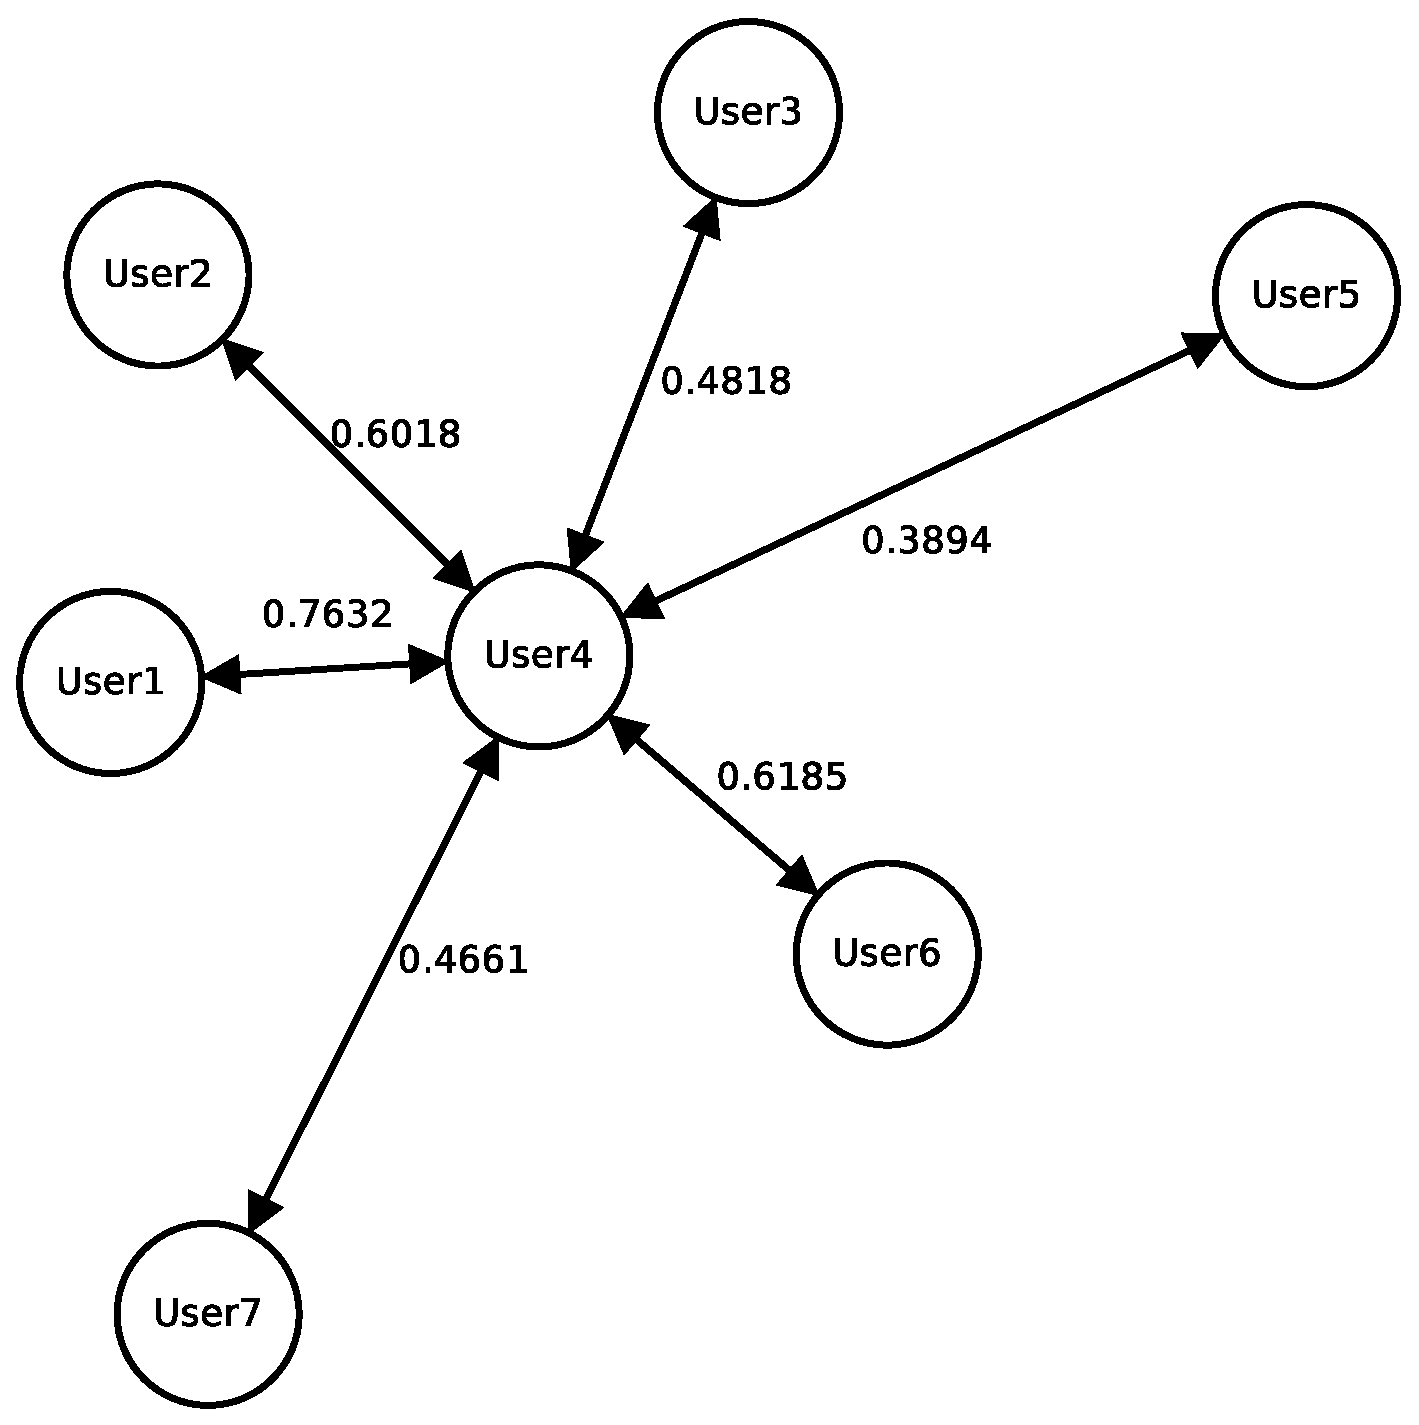
\includegraphics[width=0.5\textwidth]{chapter_2/KNN_example.eps}
	\caption{Cosine Similarities for $User_4$}
	\label{figure:KNN_example}
	\end{figure}
	\item[] \textbf{Step 3:}  Sort that similarities in descending order.
	\begin{align*}
		\begin{split}
			&cos(User_1, User_4) = 0.7632\\
			&cos(User_4, User_6) = 0.6185\\
			&cos(User_2, User_4) = 0.6018\\
			&cos(User_3, User_4) = 0.4818\\
			&cos(User_4, User_7) = 0.4661\\
			&cos(User_4, User_5) = 0.3894\\
		\end{split}
	\end{align*}
	\item[] \textbf{Step 4:}  Choose how many neighbors will contribute in the rating
	prediction in this case we choose for example, $\mathcal{K}=3$.
	\begin{align*}
		\begin{split}
			&cos(User_1, User_4) = 0.7632\\
			&cos(User_4, User_6) = 0.6185\\
			&cos(User_2, User_4) = 0.6018\\
		\end{split}
	\end{align*}
	\begin{figure}[H]
	\centering
	\includegraphics[width=0.5\textwidth]{chapter_2/KNN_example1.eps}
	\caption{Select top $\mathcal{K}=3$ similar users}
	\label{figure:neighbor_selection}
	\end{figure}
	\item[] \textbf{Step 5:} Predict how $User_4$ will rate $Item_4$ using the weighted sum.
	$$\hat{r}(User_4,Item_4) = \frac{0.7632*3 + 0.6018*2 + 0.6185*3}{0.7632 + 0.6018 + 0.6185} = 2.7$$
\end{itemize}
